\chapter{Implementation\label{chap:implementation}}

This chapter describes the specific experiments conducted with
the \textsc{SciFig-Eval} apparatus defined in
Chapter~\ref{chap:design}. The register shifts from specification
to execution: what was run, on which models, under which
conditions, and with which controls. The experiments are organised
by the research question each is designed to address.

\section{Experimental Strategy}
\label{sec:impl-strategy}

The evaluation exercises thirteen vision-language models drawn
from six families across the four research questions defined in
\S\ref{sec:intro-rqs}. Every model receives the same prompts,
the same images, and the same probe questions under the same
decoding parameters ($T{=}0$, no sampling). Every response is
scored independently by two LLM judges (GPT-4o and Mistral
Large~3, both hosted on Azure) so that inter-judge agreement can
be reported alongside the scores themselves. Where a research
question admits an ablation (prompt language, chain-of-thought),
both the baseline and the ablated condition are run on the same
model--figure pairs so that the comparison is paired.

The experiments were executed between March and April~2026. All
API calls use temperature zero for reproducibility. Model
outputs, judge scores, and aggregated results are versioned in
the project repository and served to the interactive dashboard
described in \S\ref{sec:impl-infra}.
Table~\ref{tab:environment} summarises the execution environment
and the reproducibility controls applied throughout.

\begin{table}[tbp]
  \centering
  \small
  \caption[Execution environment and reproducibility controls.]{%
    Execution environment and reproducibility controls.}
  \label{tab:environment}
  \setlength{\tabcolsep}{5pt}
  \begin{tabular}{@{}ll@{}}
    \toprule
    Component & Configuration \\
    \midrule
    \multicolumn{2}{@{}l}{\textit{Local execution environment}} \\
    Operating system      & macOS Darwin 25.1.0 (Apple Silicon) \\
    Python version        & 3.9+ \\
    Orchestration         & custom Python scripts, ThreadPoolExecutor \\
    Parallelism           & 4 workers per experiment \\
    \midrule
    \multicolumn{2}{@{}l}{\textit{Azure OpenAI}} \\
    Region                & East US 2 \\
    API version           & 2024-12-01-preview \\
    Deployments           & gpt-5-2, phi-4-multimodal, gpt-4o, mistral-large-3 \\
    \midrule
    \multicolumn{2}{@{}l}{\textit{OpenRouter}} \\
    Endpoint              & \texttt{openrouter.ai/api/v1} \\
    Models hosted         & 11 models (see Table~\ref{tab:models}) \\
    \midrule
    \multicolumn{2}{@{}l}{\textit{Reproducibility controls}} \\
    Temperature           & 0 (all generation and judge calls) \\
    Random seed           & deterministic (no sampling) \\
    Output format         & structured JSON per figure \\
    Version control       & Git, all outputs committed \\
    Judge panel           & dual-judge (GPT-4o + Mistral Large 3) \\
    Inter-rater metrics   & Cohen's $\kappa$, Fleiss' $\kappa$, Cronbach's $\alpha$ \\
    Dashboard             & React/TypeScript, Azure Static Web Apps \\
    \midrule
    \multicolumn{2}{@{}l}{\textit{Public resources}} \\
    Results dashboard     & \url{https://victorious-glacier-00483810f.2.azurestaticapps.net} \\
    Annotation platform   & \url{https://figureannotate.duckdns.org/projects/15/data?tab=23} \\
    \bottomrule
  \end{tabular}
\end{table}


\section{Models and Infrastructure}
\label{sec:impl-models}

The evaluation targets thirteen vision-language models drawn
from six families and five AI laboratories, selected to span
the frontier of multimodal capability at the time of writing.
The selection is organised into three tiers.

The \emph{frontier closed-weight} tier comprises three models
whose architectures are not publicly disclosed but whose
capabilities define the current state of the art:
GPT-5.2 from OpenAI \citep{openai2025gpt5},
Gemini~3.1~Pro from Google DeepMind \citep{google2026gemini3},
and Claude~Opus~4.6 from Anthropic \citep{anthropic2026opus46}.
These three models represent the highest-capability offerings
from their respective labs at the time of evaluation.

The \emph{large open-weight} tier comprises models whose
weights and technical reports are publicly available:
four members of the Qwen3-VL family from Alibaba
\citep{qwen2025qwen3vl}, spanning 8B to 235B parameters with
mixture-of-experts variants at 30B and 235B; two members of
the LLaMA-4 family from Meta \citep{meta2025llama4}, Maverick
(400B total, 17B active) and Scout (109B total, 17B active);
and three sizes of the Gemma-3 family from Google
\citep{team2025gemma3} at 4B, 12B and 27B parameters.

The \emph{small open-weight} tier is represented by
Phi-4~Multimodal from Microsoft \citep{microsoft2025phi4} at
5.6B parameters, included to test whether the A-R-I behavioural
patterns hold at the lower end of the parameter range.

Table~\ref{tab:models} lists the full model set with logos,
parameters and inference backends.

\begin{table}[tbp]
  \centering
  \small
  \caption[Models under test.]{%
    The thirteen models under test, grouped by family. Logos
    indicate the model family. All calls use $T{=}0$.
    Parameter counts for closed-weight models are undisclosed.
    MoE models report total and active parameters.}
  \label{tab:models}
  \setlength{\tabcolsep}{4pt}
  \begin{tabular}{@{}cllll@{}}
    \toprule
     & Model & Family & Parameters & Backend \\
    \midrule
    \raisebox{-3pt}{
\includegraphics[height=12pt]{figures/gptlogo.jpg}}
      & GPT-5.2  & OpenAI & undisclosed & Azure \\
    \midrule
    \raisebox{-3pt}{
\includegraphics[height=12pt]{figures/geminilogo.png}}
      & Gemini 3.1 Pro & Google DeepMind & undisclosed & OpenRouter \\
    \midrule
    \raisebox{-3pt}{
\includegraphics[height=12pt]{figures/claudelogo.png}}
      & Claude Opus 4.6 & Anthropic & undisclosed & OpenRouter \\
    \midrule
    \multirow{4}{*}{\raisebox{-12pt}{
\includegraphics[height=12pt]{figures/qwenlogo.png}}}
      & Qwen3-VL 235B-A22B & Alibaba & 235B (22B active) & OpenRouter \\
      & Qwen3-VL 32B       & Alibaba & 32B               & OpenRouter \\
      & Qwen3-VL 30B-A3B   & Alibaba & 30B (3B active)   & OpenRouter \\
      & Qwen3-VL 8B        & Alibaba & 8B                & OpenRouter \\
    \midrule
    \multirow{2}{*}{\raisebox{-5pt}{
\includegraphics[height=12pt]{figures/llama4logo.png}}}
      & LLaMA-4 Maverick & Meta & 400B (17B active) & OpenRouter \\
      & LLaMA-4 Scout    & Meta & 109B (17B active) & OpenRouter \\
    \midrule
    \multirow{3}{*}{\raisebox{-8pt}{
\includegraphics[height=12pt]{figures/gemmalogo.png}}}
      & Gemma-3 27B & Google & 27B & OpenRouter \\
      & Gemma-3 12B & Google & 12B & OpenRouter \\
      & Gemma-3 4B  & Google & 4B  & OpenRouter \\
    \midrule
    \raisebox{-3pt}{
\includegraphics[height=12pt]{figures/philogo.png}}
      & Phi-4 Multimodal & Microsoft & 5.6B & Azure \\
    \bottomrule
  \end{tabular}
\end{table}

Two inference backends are used. Azure OpenAI hosts GPT-5.2
and Phi-4 Multimodal as managed deployments. OpenRouter proxies
the remaining eleven models (including Gemini~3.1~Pro) through
a unified OpenAI-compatible endpoint. The
\texttt{FigureAnnotator} abstraction in the codebase routes each
model to its backend transparently, so every experiment script
is backend-agnostic.

\label{sec:impl-infra}
The evaluation pipeline produces structured JSON outputs at
every stage (generation, judge scoring, aggregation). A React
and TypeScript dashboard, deployed on Azure Static Web Apps,
consumes these outputs and provides interactive exploration of
per-figure, per-model, per-language results. Figure images are
served from Azure Blob Storage. The dashboard is publicly
accessible and updated after each experimental run.


\section{RQ1: Faithful Figure Description across Languages}
\label{sec:impl-rq1}

The first research question asks to what extent current VLMs
produce accurate, complete and clearly expressed descriptions
of scientific figures across typologically diverse languages.

\subsection{Experiment: Original-Image Description}
\label{sec:impl-rq1-original}

Each of the thirteen models describes all 120~sample figures
(30~Bulgarian, 30~Chinese, 39~English and multi-language,
21~German) under the native-language prompt condition (C1 in
Figure~\ref{fig:prompt-engineering}). The model receives the
clean, uncropped figure image and the figure-type-specific
prompt in the figure's native language. No caption and no paper
title are provided, isolating the model's capacity to read the
image without textual scaffolding.

Figure~\ref{fig:german023-example} reproduces
\texttt{german\_fig\_023}, a stacked bar chart of public
investment by level of government as a share of GDP, which
serves as the running example throughout this chapter. The
three prompt-condition extracts beneath it illustrate conditions
C1, C2 and C2$'$ on the same figure. Full prompts for all
figure types and languages are reproduced in
Appendix~\ref{app:prompts}.

\begin{figure}[!tbp]
  \centering
  \framedfig{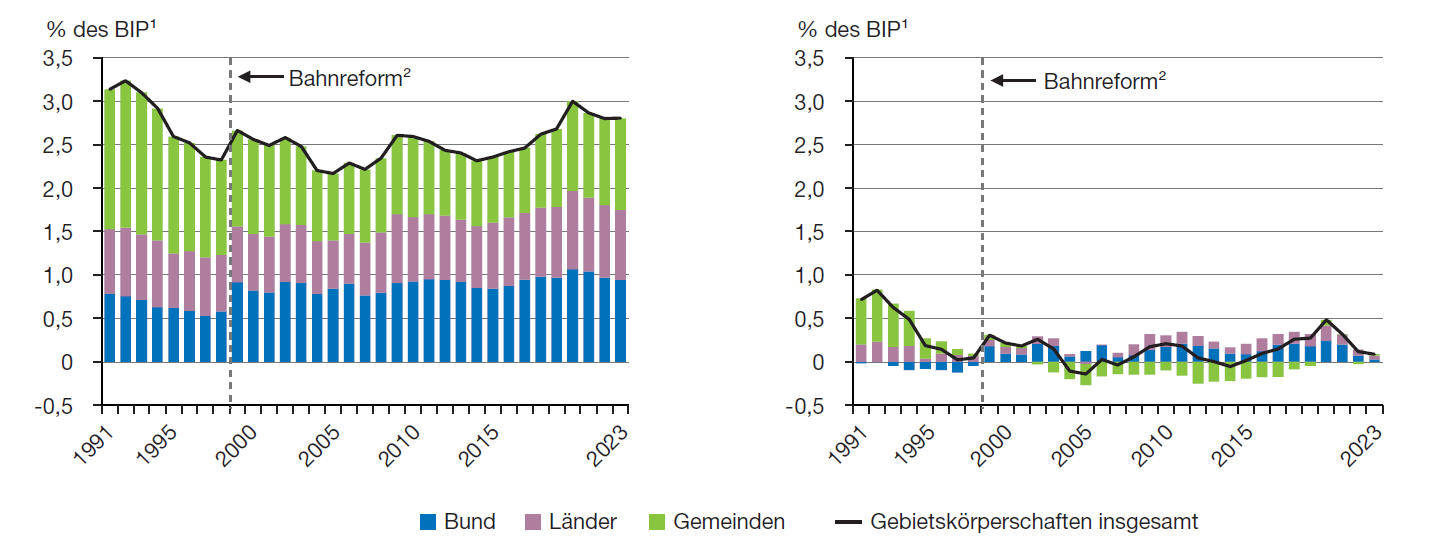
\includegraphics[width=0.75\textwidth]{figures/german_fig_023_original.png}}

  \vspace{0.6em}

  \noindent
  \begin{minipage}[t]{0.32\textwidth}
    \begin{tcolorbox}[
      enhanced, sharp corners, boxrule=0.3pt,
      colback=green!4, colframe=green!30!black!20,
      fonttitle=\sffamily\fontsize{6.5}{8}\selectfont\bfseries,
      coltitle=green!40!black,
      title={C1: Native prompt (German)},
      left=4pt, right=4pt, top=3pt, bottom=3pt]
      \fontsize{7}{9}\selectfont\itshape
      \makebox[8pt][r]{\color{codecomment}\ttfamily\upshape\fontsize{5}{6}\selectfont 1\;}%
      Sie sind ein Annotator, dessen Aufgabe es ist,
      wissenschaftliche Balkendiagramme in einem
      strukturierten, aber nat\"{u}rlichen Absatzformat
      zu beschreiben.
      \makebox[8pt][r]{\color{codecomment}\ttfamily\upshape\fontsize{5}{6}\selectfont 5\;}%
      Ihr Ziel ist es, das Dargestellte
      objektiv zu beschreiben\,\ldots
    \end{tcolorbox}
  \end{minipage}\hfill
  \begin{minipage}[t]{0.32\textwidth}
    \begin{tcolorbox}[
      enhanced, sharp corners, boxrule=0.3pt,
      colback=blue!4, colframe=blue!30!black!20,
      fonttitle=\sffamily\fontsize{6.5}{8}\selectfont\bfseries,
      coltitle=blue!40!black,
      title={C2: English prompt},
      left=4pt, right=4pt, top=3pt, bottom=3pt]
      \fontsize{7}{9}\selectfont\itshape
      \makebox[8pt][r]{\color{codecomment}\ttfamily\upshape\fontsize{5}{6}\selectfont 1\;}%
      You are an annotator tasked with describing scientific
      bar charts in a structured but natural paragraph format.
      \makebox[8pt][r]{\color{codecomment}\ttfamily\upshape\fontsize{5}{6}\selectfont 5\;}%
      Your goal is to objectively describe what is
      shown\,\ldots
    \end{tcolorbox}
  \end{minipage}\hfill
  \begin{minipage}[t]{0.32\textwidth}
    \begin{tcolorbox}[
      enhanced, sharp corners, boxrule=0.3pt,
      colback=purple!4, colframe=purple!30!black!20,
      fonttitle=\sffamily\fontsize{6.5}{8}\selectfont\bfseries,
      coltitle=purple!40!black,
      title={C2$'$: English instr.\ + native out},
      left=4pt, right=4pt, top=3pt, bottom=3pt]
      \fontsize{7}{9}\selectfont\itshape
      \makebox[8pt][r]{\color{codecomment}\ttfamily\upshape\fontsize{5}{6}\selectfont 1\;}%
      You are an annotator tasked with describing scientific
      bar charts in a structured but natural paragraph
      format\,\ldots\par
      \vspace{3pt}
      \upshape\fontseries{b}\selectfont
      \makebox[8pt][r]{\color{codecomment}\ttfamily\fontsize{5}{6}\selectfont n\;}%
      IMPORTANT: Write your response in German (Deutsch).
    \end{tcolorbox}
  \end{minipage}

  \caption[Running example: \texttt{german\_fig\_023} with three prompt conditions.]{%
    Running example used throughout this chapter.
    \texttt{german\_fig\_023} is a stacked bar chart from
    Wirtschaftsdienst showing gross and net fixed-asset
    investment by Bund (blue), L\"{a}nder (red) and
    Gemeinden (yellow) as a share of GDP, 1991--2023.
    Beneath: the opening lines of the three prompt
    conditions. C1~(green) is the native German prompt.
    C2~(blue) is the English-only ablation. C2$'$~(purple)
    uses the English prompt but appends an explicit
    instruction to respond in German.}
  \label{fig:german023-example}
\end{figure}

The resulting descriptions are evaluated under the atomic MQM
rubric defined in \S\ref{sec:design-scoring}. The judge
receives the original image, the atom checklist (2{,}252~atoms
across 120~figures, each tagged with a severity of Critical,
Important or Minor), and the model's description, and verifies
each atom independently. The normalized scoring formula
$\mathrm{MQM} = \max(0,\; 100 - (\sum\mathrm{penalties}\,/\,
N_{\mathrm{atoms}} \times 5.0) \times 100)$ ensures the full
$[0, 100]$ range is reachable regardless of figure complexity.
Both judges (GPT-4o and Mistral Large~3) score every
description independently, yielding two evaluations per model
per figure.

\subsection{Experiment: Prompt-Language Ablation}
\label{sec:impl-rq1-ablation}

To isolate the contribution of native-language prompting, two
ablation conditions are tested on the 45~adversarial-subset
figures across all thirteen models.

The first ablation uses English prompts with English output
(condition~C2). The English prompt for each figure type is used
regardless of the figure's native language, and the model
responds in English. This changes both the instruction language
and the output language relative to condition~C1.

The second ablation uses English prompts but explicitly requests
native-language output. The English prompt is appended with an
instruction such as ``Write your response in Bulgarian'' (or the
corresponding directive for Chinese and German). This isolates
the instruction-language effect from the output-language effect:
if C2 scores lower than C1, the second ablation reveals whether
the drop is caused by the English instruction, the English
output, or both.

Both ablation conditions are evaluated under the same atomic
MQM rubric and by the same judge panel as the baseline, so
the per-language score differences are paired comparisons on
the same model--figure pairs.


\section{RQ2: Robustness to Visual Degradation}
\label{sec:impl-rq2}

The second research question asks how visual degradation affects
the accuracy, completeness and clarity of VLM-generated figure
descriptions. For this question, 45~figures are further sampled
from the 120-figure corpus (9~per language subset) and subjected
to controlled visual perturbations.

\subsection{Experiment: Image Transforms}
\label{sec:impl-rq2-transforms}

Each of the 45~adversarial figures is transformed under seven
degradation conditions drawn from probe family~A3: JPEG
compression ($q{=}15$), Gaussian noise ($\sigma{=}30$),
aspect-ratio stretch (${\times}1.2$), contrast reduction
(${\times}0.5$), thirty-degree rotation, embedding in the
original paper page (original-in-paper), and embedding in the
paper page with the figure region blurred (blurred-in-paper).
Figure~\ref{fig:transforms-example} illustrates three of these
transforms on the running example, showing noise injection,
rotation and blurred-in-paper embedding.

\begin{figure}[!tbp]
  \centering
  \begin{subfigure}[t]{0.32\textwidth}
    \centering
    \framedfig{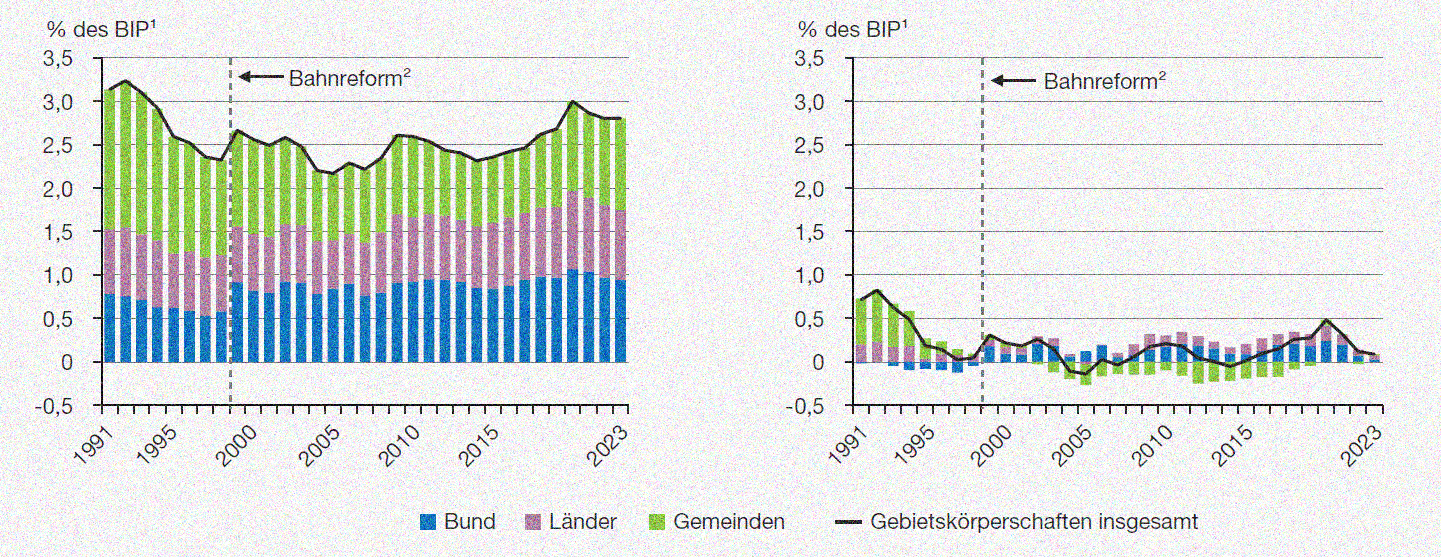
\includegraphics[width=\linewidth]{figures/german_fig_023_noise.png}}
    \caption{Gaussian noise ($\sigma{=}30$)}
  \end{subfigure}\hfill
  \begin{subfigure}[t]{0.32\textwidth}
    \centering
    \framedfig{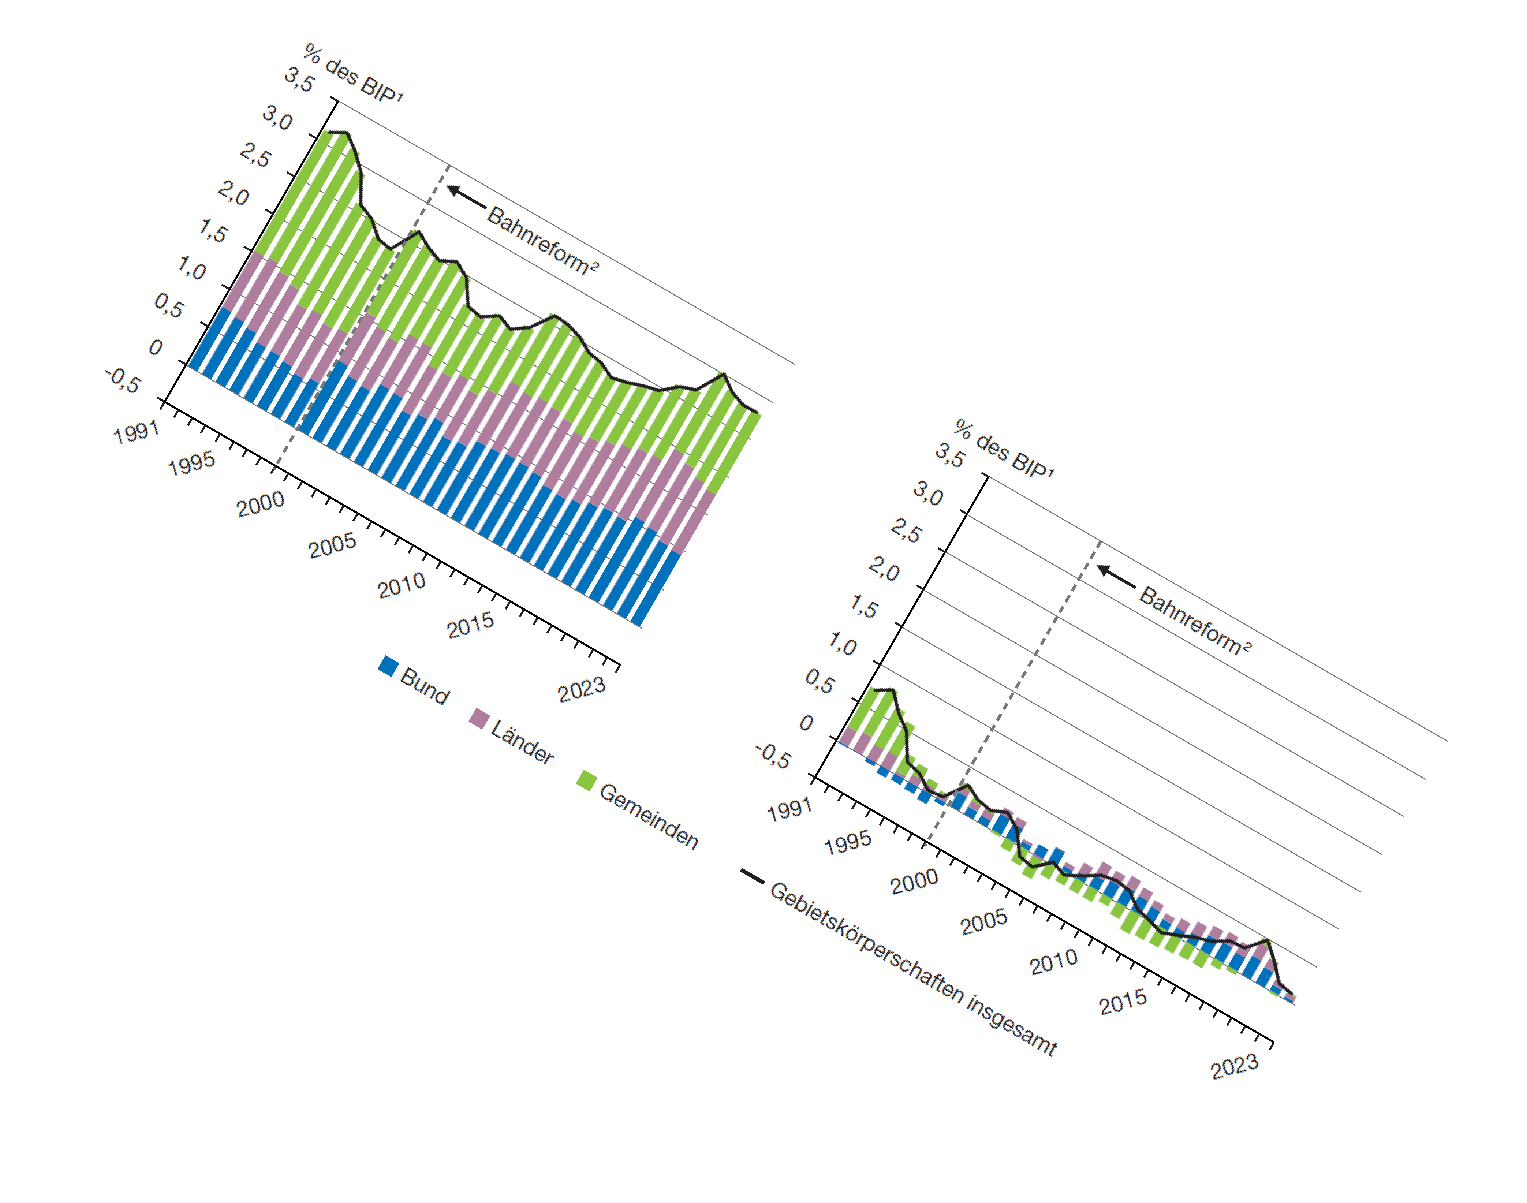
\includegraphics[width=\linewidth]{figures/german_fig_023_rotation.png}}
    \caption{Rotation ($30^{\circ}$)}
  \end{subfigure}\hfill
  \begin{subfigure}[t]{0.32\textwidth}
    \centering
    \framedfig{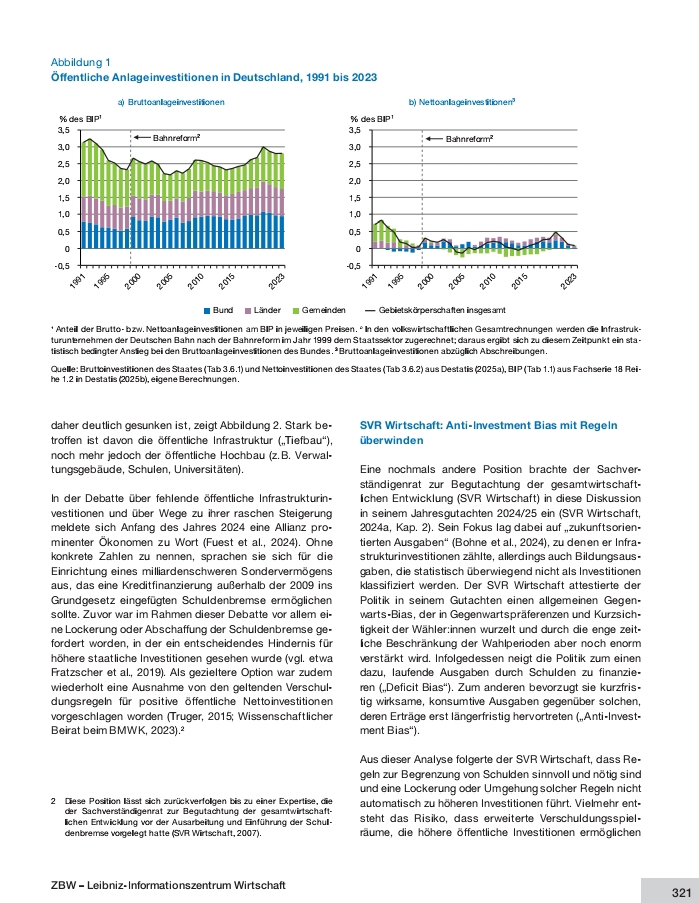
\includegraphics[width=\linewidth]{figures/german_fig_023_original_in_paper.jpeg}}
    \caption{Original in paper page}
  \end{subfigure}
  \caption[Three visual transforms applied to \texttt{german\_fig\_023}.]{%
    Three representative transforms from probe family~A3
    applied to the running example. \textbf{(a)}~Gaussian noise
    degrades fine detail while preserving gross structure.
    \textbf{(b)}~Rotation displaces axis labels from their
    expected positions. \textbf{(c)}~Original-in-paper embeds the
    figure in its original page context, testing whether the
    model can identify and describe the correct figure when
    presented alongside surrounding text and other page
    elements. Compare with the clean original in
    Figure~\ref{fig:german023-example}.}
  \label{fig:transforms-example}
\end{figure}

Every model describes every transformed figure under
condition~C1, producing $13 \times 7 \times 45 = 4{,}095$
descriptions in total (minus a small number of figures excluded
from the in-paper conditions where the page snapshot was
unavailable). Each description is evaluated under atomic MQM by
both judges. The per-transform score is compared against the
original-image baseline from \S\ref{sec:impl-rq1-original} to
quantify the degradation profile of each model.

\subsection{Experiment: Axis and Selective Blur}
\label{sec:impl-rq2-blur}

Two additional transforms target specific figure regions rather
than the image as a whole. Figure~\ref{fig:blur-example}
illustrates both on the running example.

\begin{figure}[H]
  \centering
  \begin{subfigure}[t]{0.48\textwidth}
    \centering
    \framedfig{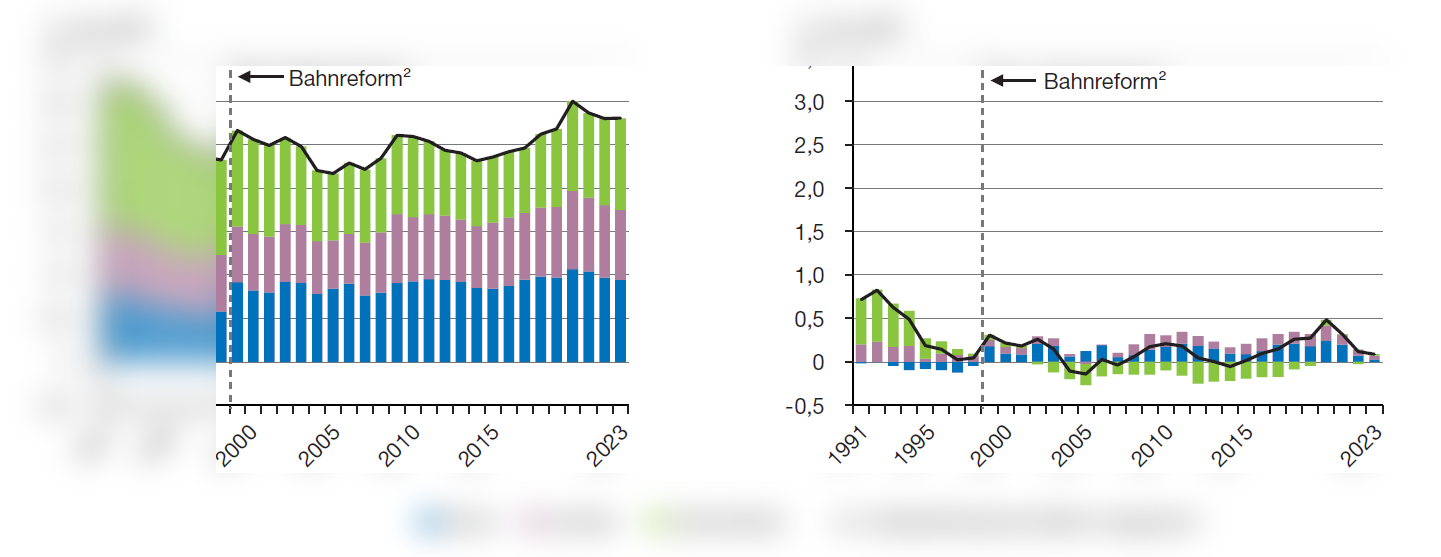
\includegraphics[width=\linewidth]{figures/german_fig_023_axis_blurred.png}}
    \caption{Axis blur}
  \end{subfigure}\hfill
  \begin{subfigure}[t]{0.48\textwidth}
    \centering
    \framedfig{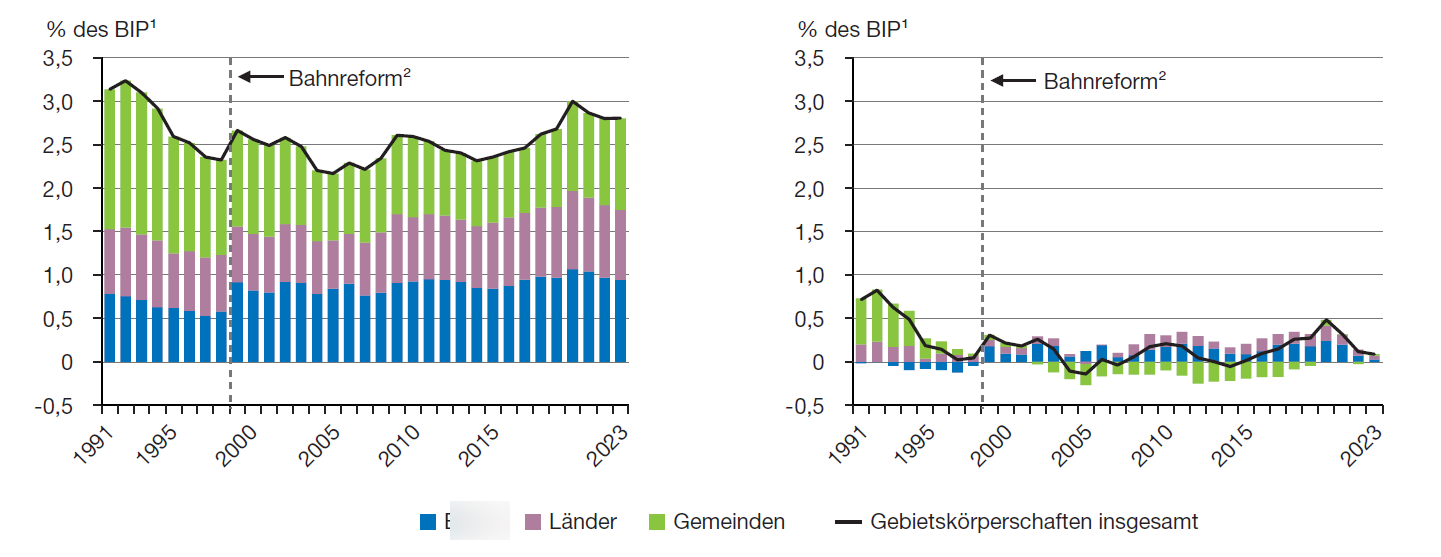
\includegraphics[width=\linewidth]{figures/german_fig_023_selective_blur.png}}
    \caption{Selective blur}
  \end{subfigure}
  \caption[Axis blur and selective blur on \texttt{german\_fig\_023}.]{%
    Region-targeted blur transforms on the running example.
    \textbf{(a)}~Axis blur applies a Gaussian blur to the top,
    left and bottom margins, obscuring axis labels and tick
    marks while leaving the data region legible.
    \textbf{(b)}~Selective blur applies a localised blur to a
    single in-chart element (here, a bar label), testing whether
    the model admits the element is unreadable or fabricates a
    value.}
  \label{fig:blur-example}
\end{figure}

Axis blur obscures axis labels and tick marks while leaving the
data region legible. Selective blur targets a single in-chart
element (a bar label, a pie-chart slice label, or a line-plot
legend entry) identified from the ground-truth annotation. The
45~figures yield 128~blurred axis elements and 47~blurred
selective elements. These blurred descriptions feed the
Admittance axis of the A-R-I framework and are evaluated under
the passive-admittance rubric described in
\S\ref{sec:design-ari-admittance}.


\section{RQ3: Comprehension beyond Description}
\label{sec:impl-rq3}

The third research question asks whether VLMs can demonstrate
genuine comprehension of scientific visualisations beyond
surface description.

\subsection{Experiment: Capability Questions}
\label{sec:impl-rq3-capability}

A set of 225~capability questions, distributed across the
five language subsets, tests quantitative reading, approximate
estimation, and open-ended interpretation of the 45~adversarial
figures. Each figure has five questions spanning three answer
types: exact (a specific number or label), approximate (a
value within a tolerance range), and open-ended (a qualitative
observation). Figure~\ref{fig:capability-questions} illustrates
the five questions for the running example. The questions are
delivered to each model in two batches of five, with each batch
also containing hallucination and prompt-reverse probes (see
\S\ref{sec:impl-rq4}). The model's answers are parsed from the
numbered response and scored by both judges against the
ground-truth answer key.

\begin{figure}[H]
  \centering
  \begin{tikzpicture}[
    font=\sffamily,
    pill/.style={rounded corners=4pt, inner xsep=5pt, inner ysep=2pt,
      font=\sffamily\fontsize{6}{7.5}\selectfont\bfseries},
    pillapx/.style={pill, fill=orange!25, text=orange!75!black},
    pillext/.style={pill, fill=blue!25, text=blue!65!black},
    pillopn/.style={pill, fill=green!30, text=green!55!black},
  ]
    \def\colw{2.7cm}
    \def\totalw{13.5cm}

    %% Cartesian axes with arrows
    \draw[-{Latex[length=2mm,width=1.5mm]}, black!60, line width=0.6pt]
      (-0.15, -5.3) -- (\totalw+0.3, -5.3);
    \draw[-{Latex[length=2mm,width=1.5mm]}, black!60, line width=0.6pt]
      (0, -5.5) -- (0, 1.1);

    %% Axis labels
    \node[font=\sffamily\fontsize{5}{6}\selectfont, text=black!40,
          anchor=south] at (0, 1.15) {type};
    \node[font=\sffamily\fontsize{5}{6}\selectfont, text=black!40,
          anchor=west] at (\totalw+0.35, -5.3) {Q};

    %% Dashed vertical partition lines
    \foreach \i in {1,...,4} {
      \draw[dashed, black!30, line width=0.4pt]
        (\i*\colw, 0.9) -- (\i*\colw, -5.3);
    }

    %% === Q1 ===
    \node[pillapx] at (0.5*\colw, 0.55) {Approximate};
    \node[font=\sffamily\fontsize{8}{9}\selectfont\bfseries,
          text=black] at (0.5*\colw, -0.15) {Q1};
    \node[font=\sffamily\fontsize{6}{8}\selectfont,
          text=black!90, text width=2.3cm, align=center]
          at (0.5*\colw, -1.5) {\itshape
          In welchem unge\-f\"{a}hren Jahr erreichen die Brutto\-anlage\-investitionen ihren h\"{o}chsten Wert?};
    \node[font=\sffamily\fontsize{5}{6.5}\selectfont,
          text=black!50, text width=2.3cm, align=center]
          at (0.5*\colw, -3.1) {%
          In what approximate year do gross investments reach their peak?};
    \node[font=\sffamily\fontsize{5.5}{7}\selectfont\bfseries,
          text=orange!70!black, text width=2.3cm, align=center]
          at (0.5*\colw, -4.3) {$\approx$1992--93\\3.3\% GDP};

    %% === Q2 ===
    \node[pillapx] at (1.5*\colw, 0.55) {Approximate};
    \node[font=\sffamily\fontsize{8}{9}\selectfont\bfseries,
          text=black] at (1.5*\colw, -0.15) {Q2};
    \node[font=\sffamily\fontsize{6}{8}\selectfont,
          text=black!90, text width=2.3cm, align=center]
          at (1.5*\colw, -1.5) {\itshape
          In welchen Jahren fallen die Netto\-anlage\-investitionen unter 0\% des BIP?};
    \node[font=\sffamily\fontsize{5}{6.5}\selectfont,
          text=black!50, text width=2.3cm, align=center]
          at (1.5*\colw, -3.1) {%
          In which years do net investments fall below 0\% of GDP?};
    \node[font=\sffamily\fontsize{5.5}{7}\selectfont\bfseries,
          text=orange!70!black, text width=2.3cm, align=center]
          at (1.5*\colw, -4.3) {$\approx$2003--2014};

    %% === Q3 ===
    \node[pillapx] at (2.5*\colw, 0.55) {Approximate};
    \node[font=\sffamily\fontsize{8}{9}\selectfont\bfseries,
          text=black] at (2.5*\colw, -0.15) {Q3};
    \node[font=\sffamily\fontsize{6}{8}\selectfont,
          text=black!90, text width=2.3cm, align=center]
          at (2.5*\colw, -1.5) {\itshape
          Wie gro\ss{} ist die Differenz zwischen Brutto- und Netto\-investitionen 2023?};
    \node[font=\sffamily\fontsize{5}{6.5}\selectfont,
          text=black!50, text width=2.3cm, align=center]
          at (2.5*\colw, -3.1) {%
          How large is the gap between gross and net investment in 2023?};
    \node[font=\sffamily\fontsize{5.5}{7}\selectfont\bfseries,
          text=orange!70!black, text width=2.3cm, align=center]
          at (2.5*\colw, -4.3) {$\approx$2.6--2.75\\pct.\ points};

    %% === Q4 ===
    \node[pillext] at (3.5*\colw, 0.55) {Exact};
    \node[font=\sffamily\fontsize{8}{9}\selectfont\bfseries,
          text=black] at (3.5*\colw, -0.15) {Q4};
    \node[font=\sffamily\fontsize{6}{8}\selectfont,
          text=black!90, text width=2.3cm, align=center]
          at (3.5*\colw, -1.5) {\itshape
          Welche Gebietsk\"{o}rper\-schafts\-ebene hat durchgehend den gr\"{o}\ss{}ten Anteil?};
    \node[font=\sffamily\fontsize{5}{6.5}\selectfont,
          text=black!50, text width=2.3cm, align=center]
          at (3.5*\colw, -3.1) {%
          Which level of government consistently has the largest share?};
    \node[font=\sffamily\fontsize{5.5}{7}\selectfont\bfseries,
          text=blue!65!black, text width=2.3cm, align=center]
          at (3.5*\colw, -4.3) {Gemeinden};

    %% === Q5 ===
    \node[pillopn] at (4.5*\colw, 0.55) {Open-ended};
    \node[font=\sffamily\fontsize{8}{9}\selectfont\bfseries,
          text=black] at (4.5*\colw, -0.15) {Q5};
    \node[font=\sffamily\fontsize{6}{8}\selectfont,
          text=black!90, text width=2.3cm, align=center]
          at (4.5*\colw, -1.5) {\itshape
          In welchem Jahr ist die ``Bahnreform''-Linie, und was \"{a}ndert sich danach?};
    \node[font=\sffamily\fontsize{5}{6.5}\selectfont,
          text=black!50, text width=2.3cm, align=center]
          at (4.5*\colw, -3.1) {%
          In what year is the ``Bahnreform'' line, and what changes after?};
    \node[font=\sffamily\fontsize{5.5}{7}\selectfont\bfseries,
          text=green!55!black, text width=2.3cm, align=center]
          at (4.5*\colw, -4.3) {$\approx$1998--99\\Bund share drops};

    %% Outer frame
    \begin{scope}[on background layer]
      \coordinate (bg_sw) at ($(current bounding box.south west)+(-0.1,-0.15)$);
      \coordinate (bg_ne) at ($(current bounding box.north east)+(0.1,0.1)$);
      \fill[white] (bg_sw) rectangle (bg_ne);
      \draw[black!20, line width=0.3pt, rounded corners=3pt]
            (bg_sw) rectangle (bg_ne);
    \end{scope}
  \end{tikzpicture}
  \caption[Capability questions for \texttt{german\_fig\_023}.]{%
    The five capability questions assigned to the running
    example (\texttt{german\_fig\_023},
    Figure~\ref{fig:german023-example}), shown on a five-column
    Cartesian layout. Each column shows a pill-shaped answer-type
    tag (orange for approximate, blue for exact, green for
    open-ended), the German question in italics, a faint English
    translation, and the expected answer. Every figure in the
    45-figure adversarial subset receives its own set of five
    questions in its native language, following the same
    three-type distribution.}
  \label{fig:capability-questions}
\end{figure}

\section{RQ4: Behavioural Dynamics under Stress}
\label{sec:impl-rq4}

The fourth research question asks how VLMs behave when the
visual evidence or its accompanying context is stressed. This
section covers the adversarial probes that feed all three axes
of the A-R-I framework, including inductance probes (moved here
from RQ3 because they test behavioural responses to reasoning
traps rather than straightforward comprehension) and the
chain-of-thought ablation that tests whether explicit visual
reasoning changes model behaviour under stress.

\subsection{Experiment: Hallucination Probes}
\label{sec:impl-rq4-hallucination}

Three hallucination sub-types are tested across the
45~adversarial figures. \emph{Inexist} probes ask about a
visual element that does not appear in the figure (e.g.,
``What percentage does the Anime Characters subcategory
occupy?'' on a chart that contains no such category).
\emph{Contra} probes build on a false numerical premise and
invite the model to elaborate (e.g., asserting that a bar
shows 60\% when it shows 45\%). \emph{Unanswerable} probes
ask about information the figure does not determine (e.g.,
the causal mechanism behind a trend). Each probe is scored on
a three-point scale ($1.0$ for correct refusal, $0.5$ for
hedged response, $0.0$ for confident fabrication).

\subsection{Experiment: Caption Bias}
\label{sec:impl-rq4-caption}

Each of the 45~figures is paired with a modified caption drawn
from probe family~A2. The modified caption contains one or more
factual claims that contradict the visual evidence. Each model
describes the figure twice: once with the misleading caption
(modified-caption condition) and once with no caption at all
(image-only condition). The judge compares the two descriptions
against the ground truth and classifies each factual claim as
following the image, following the caption, or not addressed.
The resistance score is the proportion of claims that follow
the image.

\subsection{Experiment: Prompt-Reverse Consistency}
\label{sec:impl-rq4-reverse}

Each figure is associated with a true statement and its logical
negation. The model is asked in separate turns to confirm the
true statement and to confirm the false statement. A model that
agrees with both is sycophantic by construction. The consistency
score is $1.0$ when the model confirms the true claim and denies
the false one, $0.5$ when it reverses (confirms false, denies
true), and $0.0$ when it agrees with both or disagrees with
both.

\subsection{Experiment: Active Admittance}
\label{sec:impl-rq4-admittance}

Forty-four selective-blur images are paired with a reasoning
question whose answer depends on the blurred element. The model
receives the degraded image and the question, and its response
is scored on whether it admits the element is unreadable
(admittance $= 1.0$), hedges ($0.5$), or fabricates a specific
value ($0.0$). This complements the passive-admittance scores
from \S\ref{sec:impl-rq2-blur}, which are derived from
unprompted descriptions rather than direct questions.

\subsection{Experiment: Passive Admittance}
\label{sec:impl-rq4-passive}

The axis-blur and selective-blur descriptions generated in
\S\ref{sec:impl-rq2-blur} are evaluated for passive admittance.
For each blurred element identified in the ground-truth
annotation, the judge checks whether the model's description
mentions the element, and if so, whether it admits the element
is unreadable, fabricates a value, or silently omits it. The
passive-admittance score for a model is the mean per-element
admittance across all blurred elements.

\subsection{Experiment: Inductance Probes}
\label{sec:impl-rq4-inductance}

Five inductance probes test whether a model can perform
non-trivial inductive reasoning that requires looking beyond
surface-level patterns. Each probe pairs a clean figure image
with a question whose naive answer (the one a surface-level
reader would give) is incorrect, and whose correct answer
requires noticing a subtlety such as a logarithmic scale, a
truncated axis, or raw counts mislabelled as percentages. The
probes are scored on the five-point inductance rubric defined
in \S\ref{sec:design-ari-inductance}, which rewards both
correctness and epistemic transparency.

\subsection{Experiment: Chain-of-Thought Ablation}
\label{sec:impl-rq4-cot}

To test whether explicit visual reasoning changes model
behaviour under stress, every probe from RQ3 and RQ4 is re-run
under condition~C3 (CCoT visual reasoning). The model first
describes the visual structure of the figure, then reasons step
by step before answering. The same judge scoring is applied to
the C3 responses, and the per-experiment score difference
between C1 and C3 quantifies the effect of chain-of-thought
prompting on each behavioural axis.

The CCoT ablation is run on all thirteen models. For
question-answering probes the full model response (including
the visual decomposition) is passed to the judge. For
description tasks (caption bias) only the text after the
\texttt{DESCRIPTION:} separator is evaluated.


\section{Summary of Experimental Conditions}
\label{sec:impl-summary}

Table~\ref{tab:experiment-summary} summarises the experimental
matrix. Each row is one experiment, each column indicates how
many model--figure pairs it produces and which scoring track
applies. The total number of judge calls across all experiments,
models, and judges exceeds 50{,}000.

\begin{table}[tbp]
  \centering
  \small
  \caption[Summary of experimental conditions.]{%
    Summary of experimental conditions. Each row is one
    experiment. The ``Figures'' column reports the number of
    distinct figure images evaluated. The ``Calls'' column
    reports the number of model invocations (models $\times$
    figures $\times$ conditions). The ``Scoring'' column
    indicates the evaluation track.}
  \label{tab:experiment-summary}
  \setlength{\tabcolsep}{4pt}
  \begin{tabular}{@{}llrrll@{}}
    \toprule
    RQ & Experiment & Figures & Calls & Scoring & Ablation \\
    \midrule
    1 & Original description     & 120 & 1,560 & atomic MQM & --- \\
    1 & Prompt-language ablation & 45  & 1,170 & atomic MQM & C2/C2$'$ vs C1 \\
    \midrule
    2 & Image transforms (7)    & 45  & 4,095 & atomic MQM & --- \\
    2 & Axis blur                & 45  & 585   & passive admittance & --- \\
    2 & Selective blur           & 45  & 585   & passive admittance & --- \\
    \midrule
    3 & Capability questions    & 45  & 1,170 & judge + rule-based & --- \\
    \midrule
    4 & Hallucination probes    & 45  & 1,755 & 3-point scale & --- \\
    4 & Caption bias            & 45  & 1,170 & resistance score & --- \\
    4 & Prompt reverse          & 45  & 585   & consistency score & --- \\
    4 & Active admittance       & 44  & 572   & admittance rubric & --- \\
    4 & Passive admittance      & 45  & 1,170 & admittance rubric & --- \\
    4 & Inductance probes       & 5   & 65    & inductance rubric & --- \\
    4 & CoT ablation (all probes) & 45 & 7,800+ & all tracks & C3 vs C1 \\
    \bottomrule
  \end{tabular}
\end{table}
